\subsubsection{A Brief History}
\comment{
Why are IoT gateways important?
How did it come to be?
How did it start?
Why is it now, that many companies have interest?
}
Mobile devices profoundly changed the way computers interact with each other. Technopedia defines a mobile device as a "handheld tablet or other device that is made for portability, and is therefore both compact and lightweight"\cite{WhatisaM95TechnopediaMobileDevice:online}, it includes laptops, smartphones, tables etc. When these devices became a commodity in the 90s\footnote{Back then smartphones were called personal digital assistant (PDA).}, the way we manage computing power needed to change to accommodate intensive tasks on light weight computers. As Mahadev Satyanarayanan put it "while mobile elements will undoubtedly improve in absolute ability, they will always be at a relative disadvantage."\cite{satyanarayanan2015briefHistoryIoTGateway} Back then, researchers experimented with local, remote (cloud) and mixed execution also called adaptive
cloud offload. Assessing the three variants for voice recognition, video playback and web browsing locally, the researchers found huge gains from adaptive cloud offloading with a high enough bandwidth and concluded "the convergence of mobile computing and cloud computing enables new multimedia applications that are both resource-intensive and interaction-intensive."\cite{noble1997agileIoTGatewayOdyssey}. This lead to an explosion in cloud development. The Internet started out with a decentralized servers around the world. But over the years technologies were invented for orchestration across these distant servers, but also isolation for the local deployments. Probably the two main technological standards evolving where containers with containerd and orchestration with Kubernetes. \\
Traditionally, mobile devices connected to a gateway, which was mainly a router operating at L3\footnote{L3 stands for Layer 3, the networking layer in the OSI model.} to route packets and translate between different types of network protocols. \cite{lee2017futureOfIoT}. However, according to Dejan Bosanac, a senior software engineer at Red Hat in the field of cloud messaging and IoT platforms, due to their proximity to the sensors and the end user, these devices have three main advantages over the cloud: 
\begin{displayquote}
{\textbf{``Low latency, availability and locality''}}\cite{IntroducingDejanBosanac:KubernetesIoTEdgeWorkingGroup} - Dejan Bosanac.
\end{displayquote}
Because of these advantage researchers construct hybrid systems, in which devices operating on the edge of the network play an active role in the data processing pipeline. This architectural style of carrying out substantial amount of computation and storage at the edge is called "edge computing" \cite{fogComputing:def}. \Cref{fig:iotDeviceSetup} shows where the gateway is positioned in the current communication setup. 
 \begin{figure}[!h]
     \centering
     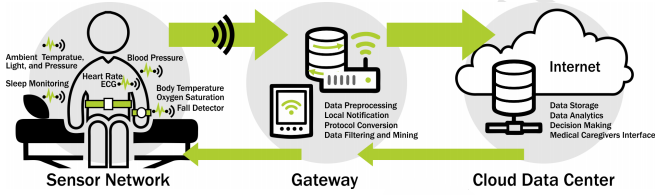
\includegraphics[scale=1.8]{figures/iotSetup.png}
     \caption{The position of the gateway in the current Internet infrastructure\cite{iotGatewaySlavesGraph}.}
     \label{fig:iotDeviceSetup}
 \end{figure}\\
But not everyone in the academic world was convinced that edge computing was indeed the way forward. In 2009, the National Science Foundation rejected a paper because \textit{``Many panelists do not agree with the premise of the proposal in which distant cloud computing incurs too high latency to be acceptable by mobile applications. They question the validity of such assumption as the proposal provides no real data to justify it[...]''}\cite{satyanarayanan2015briefHistoryIoTGateway}. Much has changed since then. The smartphone revolution (do I need to cite this? Is it a term I can actually use?) greatly increased the data produced by mobile devices and the need for speed and privacy. Researches did not foresee the explosion in IoT and the onset of a new wave data producers bundled under the term Indutrial IoT (IIoT). It includes hundreds and thousands of IoT devices working together, for example in factories, logistic warehouses, connected vehicles (CV), smart grid etc. In 2012 a widely cited paper "Fog Computing and Its Role in the Internet of Things"\cite{fogComputing:def} was published, establishing the need for IoT gateways connected to the cloud. The amount and high frequency of produced data is just too much to only handle in the cloud. Pre-processing on the edge is needed for both latency and efficiency.\\
However, establishing the need for edge computing is not the same as solving all problems though, and since then many papers have been published with titles such as "The Internet of Things Has a Gateway Problem"\cite{zachariah2015internetOfThingsHasGatewayProblem}. At the same time, researchers used custom IoT gateway solutions in their research and achieved impressive results. In one experiment, they achieved over 80\% performance increase in certain scenarios rightly titling their paper "From Cloud Computing to Fog Computing: Unleash the Power of Edge and End Devices"\cite{hong2017fromCloudtoIoTGatewayUnleashingTHePower}. Adding further to the problem of standardization is that IoT, especially IIoT, and mobile device have very different requirements.\\
This is the current place of the industry. There is a common agreement that fog computing is essential in the future, but no standard and open solution was developed yet. There is considerable effort in the academic world and in the industry to establish such a standard, one such initiatives is the Kubernetes IoT Edge working group under the Cloud Native Computing Foundry (CNCF). 


% \Cref{sec:problemArea}, \nameref{sec:problemArea}, will explain what challenges system designers face on the edge and why developing a standard is so hard.


























